\documentclass{article}
\usepackage{blindtext}
%Image-related packages
\usepackage{graphicx}
\usepackage{subcaption}
\usepackage[export]{adjustbox}
\usepackage{wrapfig}
%------------------------------

%Url related packages
\usepackage{hyperref}
\hypersetup{
    urlcolor=Cyan,
    }

\urlstyle{same}


%Table-related commands
\usepackage{array}
\usepackage[table]{xcolor}
\setlength{\arrayrulewidth}{1mm}
\setlength{\tabcolsep}{18pt}
\renewcommand{\arraystretch}{1.5}
\newcolumntype{s}{>{\columncolor[HTML]{AAACED}} p{3cm}}
%----------------------------------------------------

\title{Team Two Deliverable One}
\author{Cheuk Wei Lin, Meiqi Huang,Ross Heaney, Ruyun Sun, Yiqiu Wang}
\date{November 2022}

\graphicspath{{images/}}

\begin{document}

\maketitle

\section{Introduction}
Team Two's project is a load balancer. Load balancer's are widely used to reduce excessive resource consumption across servers when serving high volume traffic. Team two's load balancer application is divided into 7 classes
\begin{itemize}
    \item Server
    \item Serverpool
    \item Algorithm
    \item Client
    \item Loadbalancer
    \item Ipgenerator
    \item Transmit tool
\end{itemize}

All code, this LaTeX document included, can be found at \href{https://github.com/ross39/CS6422-LoadBalancer}{Github Repo.} 
We have gone for a loosely coupled, modular design so that code can be easily modified and changes made without the headaches associated with a tightly coupled design. We have also tried to make sensible decisions when it came to which data structures and algorithms to use. We have opted for a weighted round robin for the balancing algorithm. 

\section{Use Case}
%Include system overview 
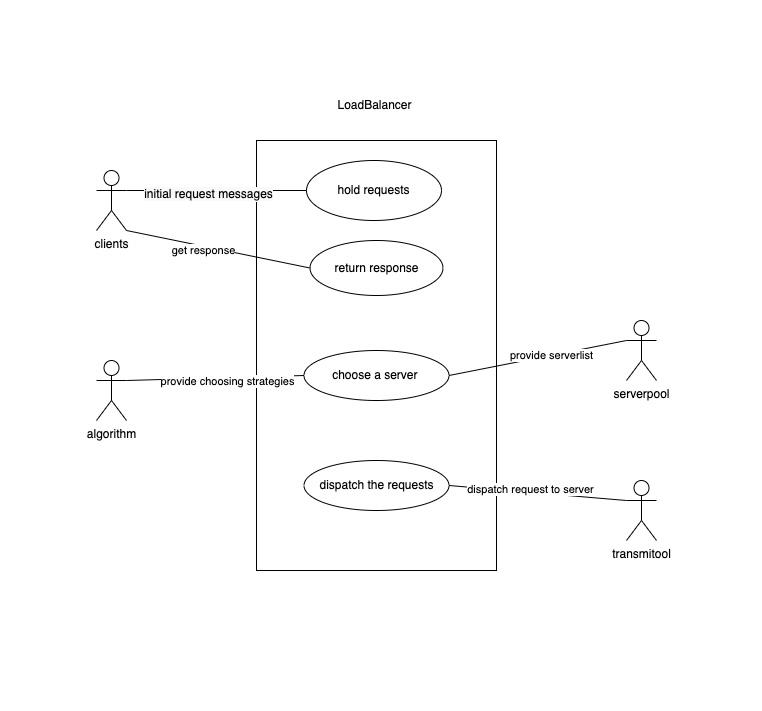
\includegraphics[width=0.7\textwidth,center]{LoadBalancer_usecase.jpeg}
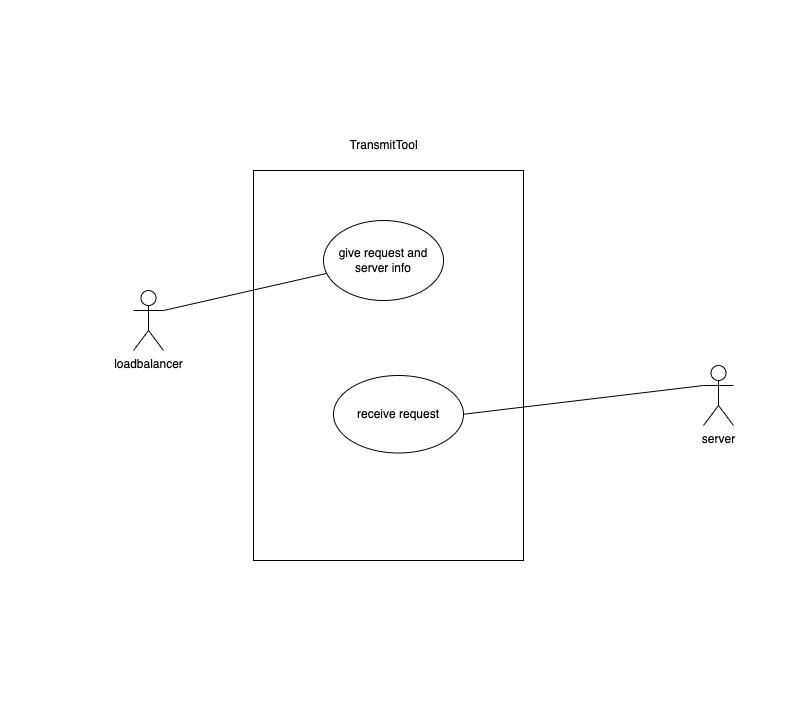
\includegraphics[width=0.7\textwidth,center]{TransmitTool_usecase.jpeg}

The client will make a request and ultimately get a response. The response will be an ip address which in the context of this load balancer, will be a link to a text file stored locally. Clients will make a lot of requests, therefore the scheduling algorithm will determine how best to route the client requests. Serverpool will maintain a list of active servers which are placed in a 'pool'. In order for a server to be considered active it will be paired with an ip address, which in this use case is just a pointer to a file on the local machine. Different servers will have different weights, these weights are an indication of how powerful a server is. Not all servers are created equally so the algorithm must take this into account when routing requests. When the request has been successfully routed, transmit tool will write to the file to indicate a successful routing of a request.

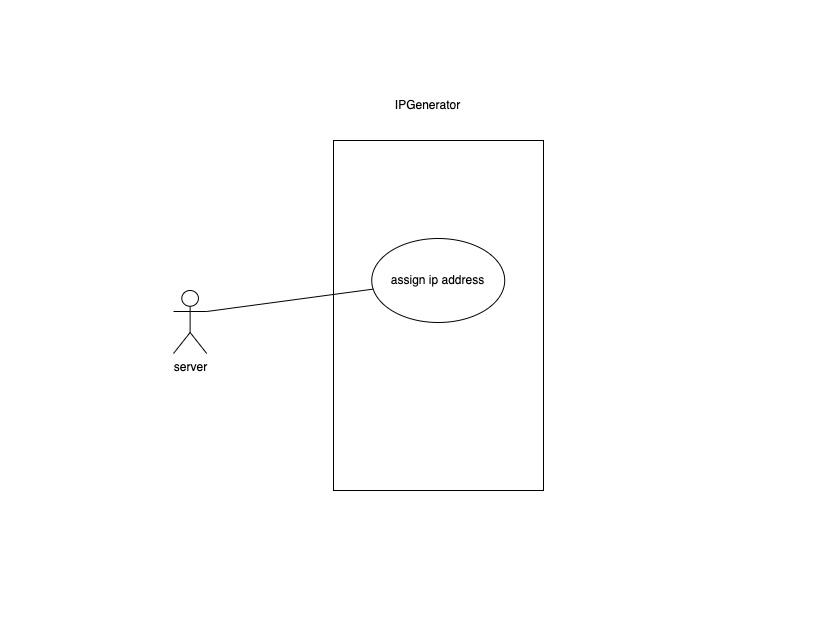
\includegraphics[width=0.7\textwidth,center]{Ipgenerator_usecase.jpeg}

Ipgenerator just generates a list of ip addresses which in this case is just a pointer to a file on the local machine. An example ip address might be 'out/ip1.txt'. The server calls ipgenerator when it needs to be paired with an ip address. We are making some simplifying instructions for this project and obviously in the real world ip addresses are a lot more complicated. 

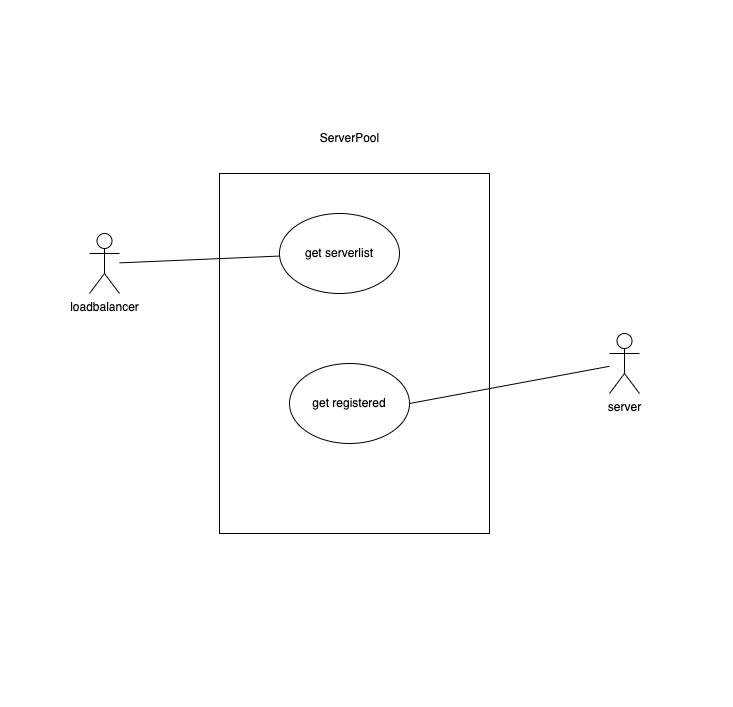
\includegraphics[width=0.7\textwidth,center]{Serverpool_usecase.jpeg}

The server will add itself to the serverpool when paired with an ip address. Once added to the serverpool this server is considered active. Serverpool will maintain a list of active servers which it will pass to loadbalancer when requested. 






\section{Requirements}
We present our list of requirements 
\begin{itemize}
    \item Log successful \& unsuccessful requests to file for transparency and diagnostics 
    \item Route client requests to the appropriate server in a timely manner. As this is being run locally we expect this to be near instantaneously.
    \item Modular \& loosely coupled design. By this we mean implementing good programming practices to ensure maintainability and testability of code.
    \item Comprehensive testing. Tests should make sense and should not be written for the sake of achieving some arbitrary test coverage. 
\end{itemize}
\subsection{Functional requirements}
This project allows users to send requests to the load balancer, and the load balancer assigns specific users to the optimal server according to the optimization algorithm to ensure that the site provides a reliable response when accepting simultaneous requests from multiple users. \\

\noindent The number of backend servers and services’ information can be updated. After logging in, the user can send a request, the load balancer receives the request and forwards the request to a currently optimal server in the server list according to the optimization algorithm. The corresponding server receives the request then start listening. \\

\subsection{Non-functional Requirements NFR's}

\textbf{Performance}: \\
The project expects that the load balancer can handle the requests of up to 50 users at the same time; After applying the load balancing algorithm, the processing time of user requests can be reduced by 70\% in the face of the same number of users accessing at the same time. \\

\noindent\textbf{Availability}: \\
The load balancer should provide 99\% SLA. \\

\noindent\textbf{Security}: \\
Communication between users, load balancers, servers is encrypted. \\

\noindent\textbf{Testability}: \\
TDD is applied to this project to ensure that the software can be evaluated.
\section{Context diagram}
%Include context diagrams
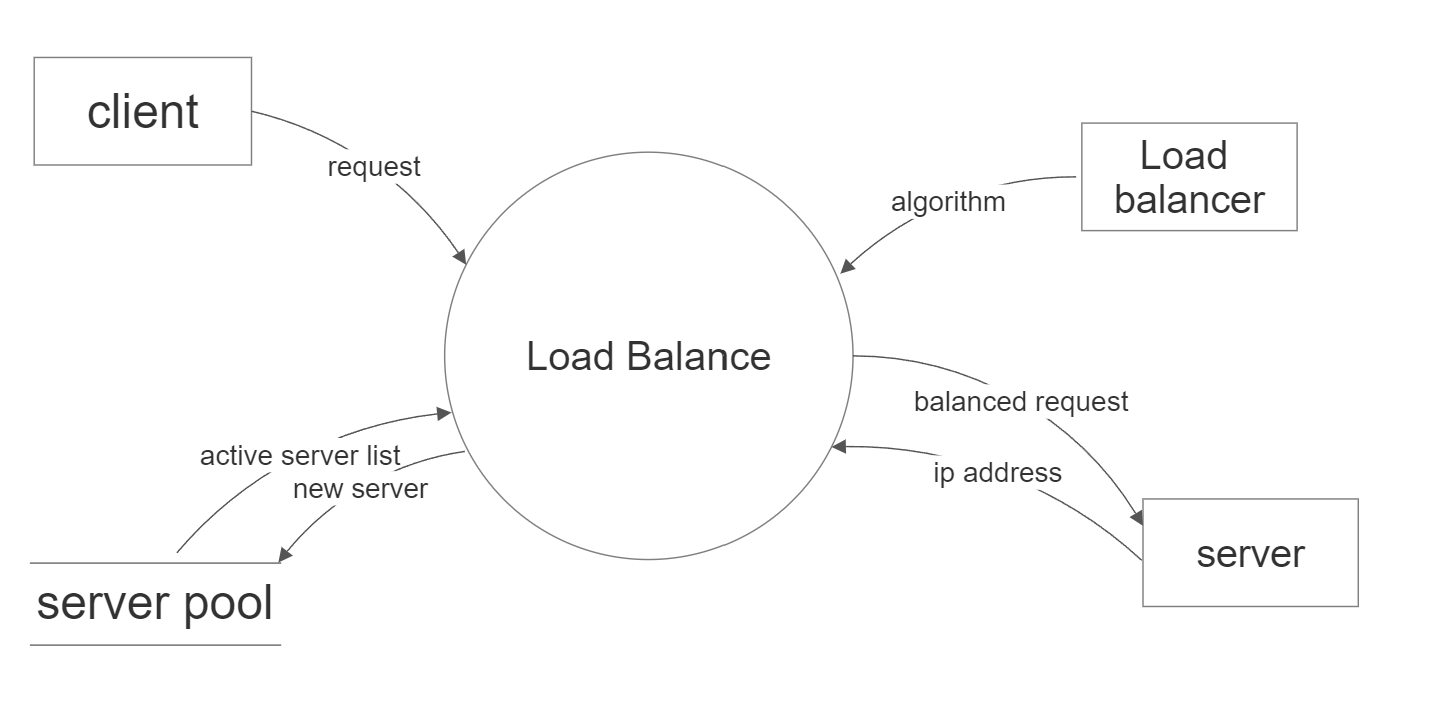
\includegraphics[width=0.7\textwidth,center]{0-level data flow diagram.png}

Essentially it is just client requests as input and the output is that a message is written to the ip address, which is a file on the local machine. In the real world the client would get a message back from the server with the content they requested but we are just simply writing a message to a file as evidence the request was successfully handled. 

\section{Data flow diagram}
%Include data flow diagrams
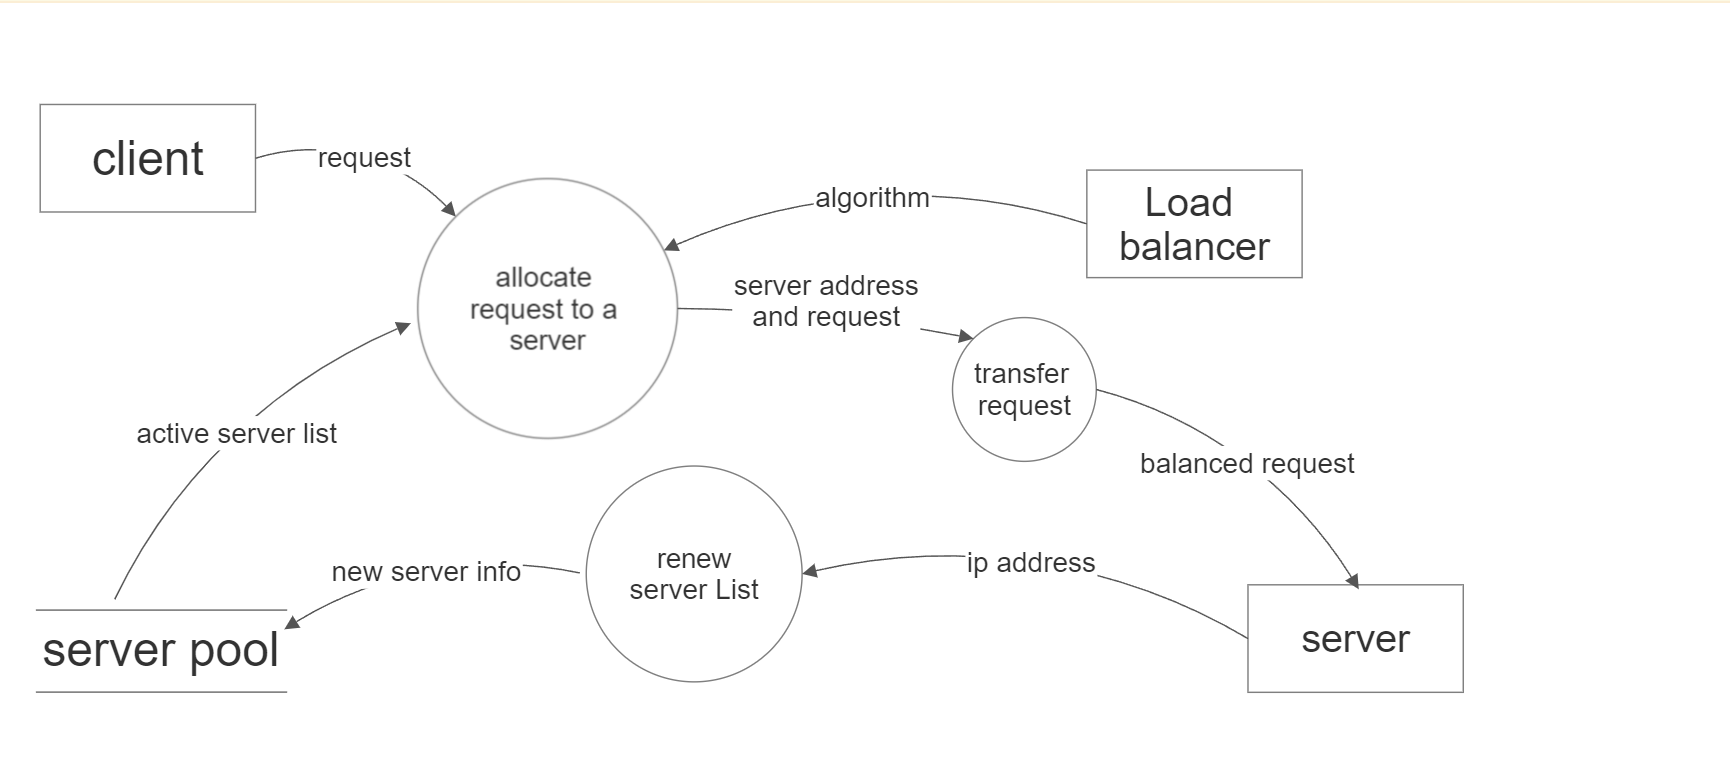
\includegraphics[width=0.7\textwidth,center]{1-level data flow diagram.png}

When the client makes a request the load balancer needs to have some information on hand to be able to handle the client request efficiently. It needs a list of active servers, which it will get from the ServerPool and it needs an algorithm, which it will get from Algorithm. This modular design means that the Algorithm can be easily swapped out if needed and the load balancer and server are loosely coupled so if changes are made to the server, the load balancer will not care provided it is given a list of active/online servers. In order for a server to the considered active, it must be paired with an ip address, which in this case is just a pointer to a text file existing on the local machine. Each server will have a weight, which is a numeric indication of the servers performance. Higher performance servers can handle more requests. The weight is purely so that the algorithm has something to do otherwise if each server was the same we could just use a queue and that wouldn't be very fun. Once paired with an ipaddress, the server will be added to the serverpool, which keeps a list of all active servers. These active servers are then given to the loadbalancer which can combine the algorithm and the list of active servers in order to route the requests in an efficient manner. Each server instance will have a unique ip address(file) so successful or unsuccessful requests will be logged to that ip address(file). 

\section{Sequence diagram}
%Include sequence diagrams
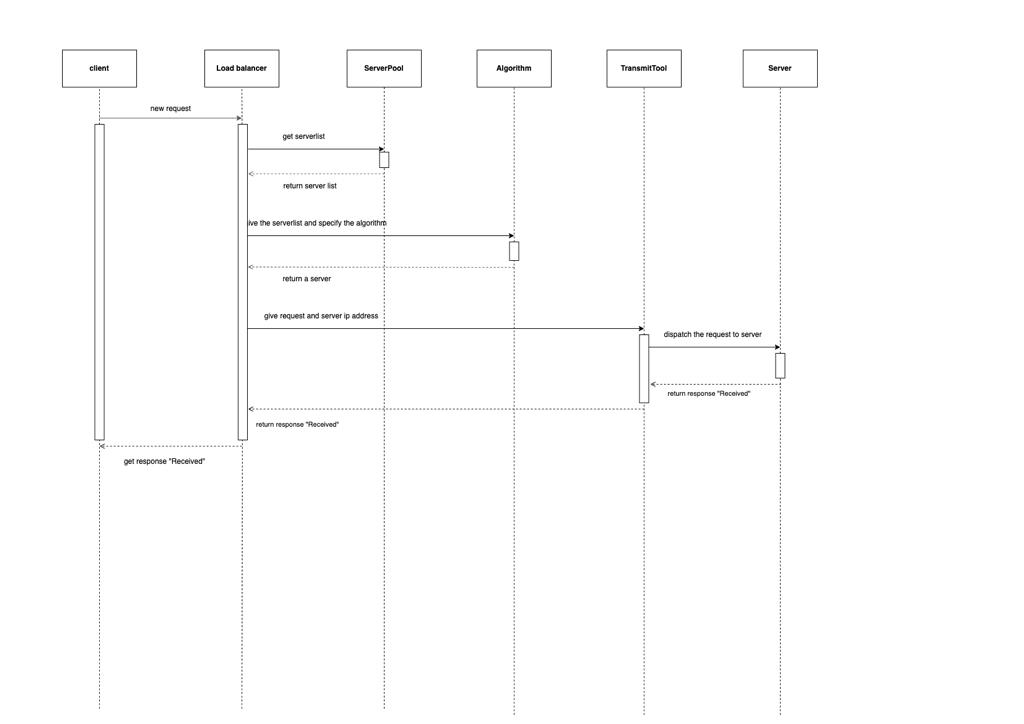
\includegraphics[width=1.5\textwidth,center]{System_sequencediagram.jpeg}

In this diagram we show the different processes taking place inside the system from when the client makes a request to when the server receives the request and a message is dispatched to show proof of request received. Firstly the client makes a request. This request is received by the load balancer. The load balancer needs some information, namely a list of active servers. The load balancer will take the serverlist and specify which algorithm it wants to use for the algorithm service. The algorithm service supports round robin and weighted round robin. The algorithm will use either round robin or weighted round robin on the serverlist, which is a list of active servers. It will then return a result to loadbalancer. Loadbalancer will pass the request to the transmit tool which sends the request to the server. To simulate this sending of the request to the server, we decided to write a message to the ip address, which is just a pointer to a text file existing on the local machine. An example of a server might be ("server1","ip1.txt") where the server is called server1 and its ip address is 1p1.txt. This ip address is represented as a string in the system so the system is completely ignorant of what it is until transmit tool takes the ip address and writes to the file. \\

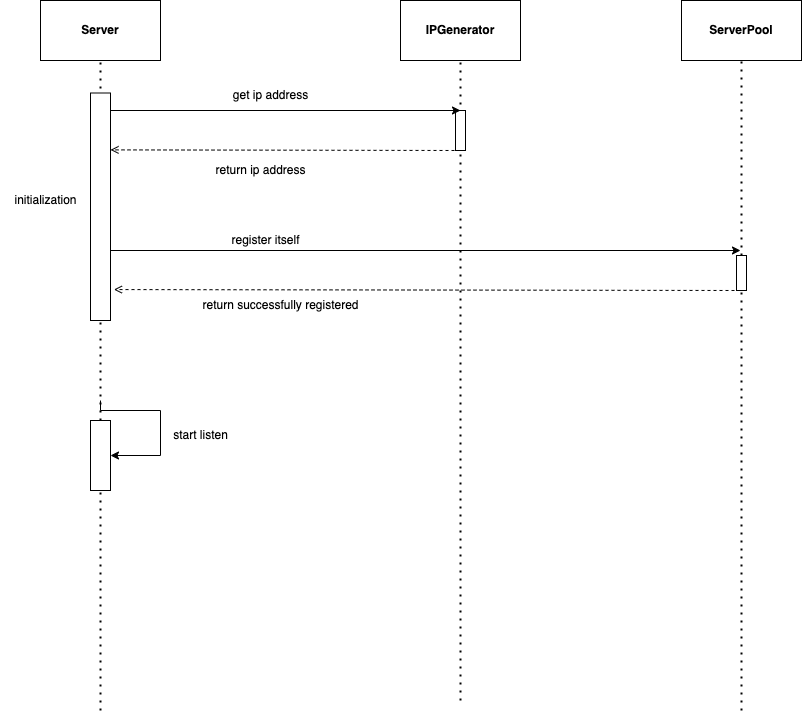
\includegraphics[width=.9\textwidth, center]{initialization-seq.jpg}
At start up, Server instances request Ip addresses from IpGenerator. These Ip addresses are then returned and now that each server instance has an ipaddress, it can be added to the serverpool. Doing this process ensures each server is registered and is paired with an ipaddress. It will then create a file according to ip address and that represents the server starts listening.

\section{Finite state machine}
%Include finite state machines
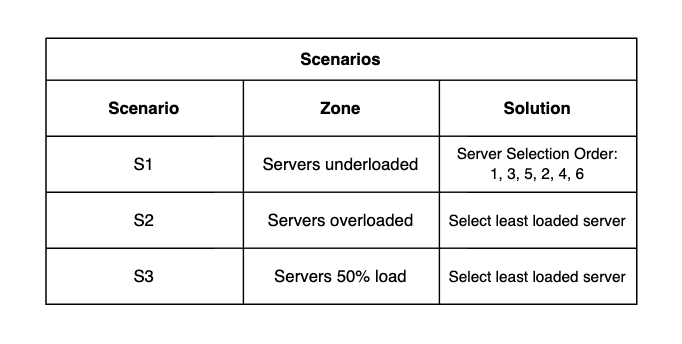
\includegraphics[width=0.7\textwidth,center]{scenarios.png}

The scenarios table depicts the possible scenarios of the server’s load. The load can vary depending on the number of client requests. Three scenarios are given in this case which includes the server being underl oaded, overloaded or at 50\% load. The load balancer will be in charge of balancing the server’s load based on the scenario. 

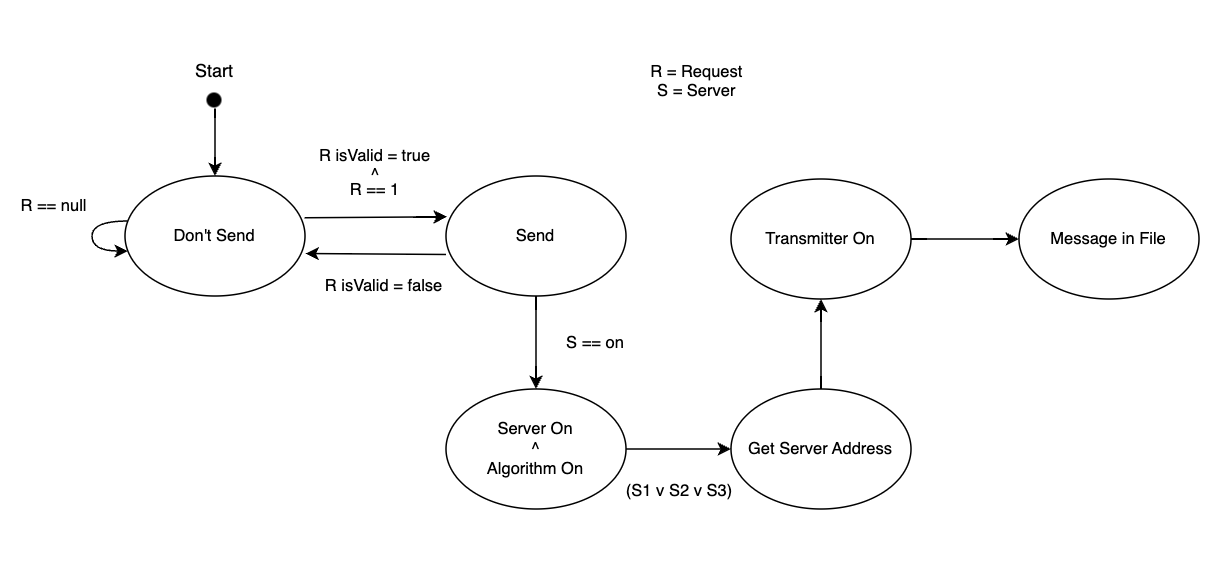
\includegraphics[width=0.7\textwidth,center]{finite-state-machine.png}

The finite state machine shows the transition from one state to another where each state performs a different action. 
Send and Don’t Send: Provided the client has a valid request, the request will be sent to the load balancer. If the request is invalid, then the request cannot be sent. 
Server and Algorithm On: The load balancer manages the list of servers and the algorithm. The client request will be allocated to an under loaded server with the aid of an algorithm to ensure the request is not issued to an overloaded server. 
Get Server Address: Once the server has been selected by the algorithm, the load balancer class will obtain the server ip address. The server ip address essentially points to a text file in the server directory. 
Transmitter On: In this state, the client request to the server will be written to a file. i.e. the server that has been selected by the algorithm

\section{Notes}
I tried to get captions on the images but I keep getting a weird error where the LaTeX would compile fine but the images appeared out of order and inbetween text. I used the following 
\begin{verbatim}

\begin{figure}[h]
\caption{Insert caption here }
\centering
\includegraphics[width=0.5\textwidth]{image}
\end{figure}
\end{verbatim}

It would format the first few images fine and then images started to be misaligned and would appear randomly half way through a paragraph of text. I will try to figure this out as its been annoying me for a while. So that is why unfortunately we are missing captions on our images. Also each sequence diagrams is corresponding to two use case diagrams.


\end{document}

